% \documentclass[a4paper]{jarticle} % 一般的なスタイルの書き方
\documentclass[a4paper,twocolumn]{ujarticle} % 2段構成のスタイル
%\documentclass[a4paper]{jreport} %卒論原稿はこのスタイル
\setlength{\topmargin}{-2.04cm}%例:上余白を設定
\setlength{\oddsidemargin}{-1.04cm}%例:左余白を1.5cmにする
\setlength{\evensidemargin}{-1.04cm}%例b:左余白を1.5cmにする
\setlength{\textwidth}{18cm}%例:一行の幅を18cmにする
\setlength{\textheight}{25cm}%例:一ページの文章の縦の長さを25cmにする
%\setlength{\textwidth}{45em}%例:一行の文字数を45文字にする(未使用)

%%%%%%%%%%%%%%%%%%%%%%%%%%
%% usepaclagae 群
%%%%%%%%%%%%%%%%%%%%%%%%%%
\usepackage{amsmath,bm} %多次元空間ベクトルRを表記するのに必要
\usepackage{amsfonts}
\usepackage{ascmac} %枠付き文章を表記するのに必
\usepackage{amssymb}
% \mathbb{R}^{l} %表記例
% \usepackage{algorithm}
% \usepackage{algorithmicx}
% \usepackage{algpseudocode}
\usepackage[dvipdfmx]{graphicx}
\usepackage[dvipdfmx]{color}
\usepackage{here} %[hbtp]の代わりに[H]と書きこむと強制的にその場所に図や表を挿入す
\pagestyle{empty}%ページ番号を表示しない

%%%%%%%%%%%%%%%%%%%%%%%%%
\newcommand{\argmax}{\mathop{\rm arg~max}\limits}
\newcommand{\argmin}{\mathop{\rm arg~min}\limits}
%%%%%%%%%%%%%%%%%%%%%%%%%


\makeatletter
\def\@maketitle{%
\begin{center}%
{\LARGE \@title \par}% タイトル
\end{center}%
\begin{flushright}%
{\large \@date}% 日付
\end{flushright}%
\begin{flushright}%%
{\large \@author}% 著者
\end{flushright}%
\par\vskip 1.5em
}
\makeatother
\title{RidgeとLassoの推定} %ここにタイトルを記入すること.
\date{2019年5月8日}
\author{大森 夢拓}

\begin{document}
\maketitle
\section{はじめに}
複雑な構造を内在する現象の分析では,多項式回帰などの説明変数に関して非線形なモデルを考える必要がある.このような複雑なモデルの推定において生じる過学習を防ぐ手法が正則化法である.本稿では正則化法の中でも,RidgeとLassoを用いた推定を紹介する.また,それらを用いて実際のデータに対して計算機実験を行った.

\section{RidgeとLassoの推定}
$i$番目($i = 1, 2, \dots, n$)のデータの目的変数を$y_i$,説明変数を$\bm{x}_i=(x_{i1}, \dots, x_{ip})^{\top} \in \mathbb{R}^p$,誤差を$\epsilon_i \sim \mathcal{N}(0, \sigma^2)$,および回帰係数を$\bm{\beta}=(\beta_0, \beta_1, \dots , \beta_p)^{\top} \in \mathbb{R}^{p+1}$として,線形回帰モデル
\begin{equation}
	y_i=\beta_0 + \beta_1 x_{i1} + \beta_2  x_{i2} + \dots + \beta_p x_{ip} + \epsilon_i
	\label{eq:linear_model_origin}
\end{equation}
を考える.パラメータベクトルの長さの概念を一般化した$L_q$ノルムに基づく正則化項を用いると,正則化最小2乗法は
\begin{equation}
	S_{\alpha}(\bm{\beta}) = \sum_{i=1}^{n}\bigl(
		y_i - (
			\beta_0 + \sum_{j=1}^{p} \beta_j {x}_{ij}
		)
	\bigr)^2 + \alpha \sum_{j=1}^{p} |\beta_j|^q
	\label{eq:extendLinearRegression}
\end{equation}
のよう記述できる.$\alpha \in \mathbb{R}^+$はモデルの複雑度を設定するハイパーパラメータであり,式\eqref{eq:extendLinearRegression} の第2項が$q=1$($L_1$ノルム)の場合をLasso,$q=2$の場合をRidgeと呼ぶ.

\subsection{Ridge}
切片を除く回帰係数の2乗和を正則化項としてとることで,説明変数間の強い相関によって生じる回帰係数の推定値の不安定性を回避する手法をRidgeという.Ridge推定量の求め方は次のようになる.

$j$番目の説明変数に関するデータの平均値$\bar{x}_j$を中心化したデータを$z_{ij}=x_{ij} - \bar{x}_j$とすると,式\eqref{eq:linear_model_origin}は次のように変形できる.
\begin{equation}
        y_i = \beta_0^* + \beta_1 z_{i1} + \dots + \beta_p z_{ip} + \epsilon_i
	\label{eq:linear_model_centering}
\end{equation}
ただし,$\beta_0^* = \beta_0 + \beta_1 \bar{x}_{1} + \dots + \beta_p \bar{x}_{p}$である.さらに,$\bm{\beta}_1 = (\beta_1, \beta_2, \dots , \beta_p)^{\top} \in \mathbb{R}^p$および$ \bm{1} = (1, 1, \dots , 1)^{\top} \in \mathbb{R}^n$と定義すると式\eqref{eq:linear_model_centering}は以下の行列形式で記述できる.
\begin{equation}
	\begin{split}
		\bm{y} &= \beta_0^* \bm{1} + Z \bm{\beta}_1 + \bm{\epsilon}\\
		Z &= \left[
                \begin{array}{ccc}
                z_{11} & \dots & z_{1p} \\
                \vdots & z_{ij} & \vdots \\
                z_{n1} & \dots & z_{np} \\
                \end{array}
                \right]
        \end{split}
	\label{eq:linear_model_mat}
\end{equation}
よって,Ridge回帰モデルは,
\begin{equation}
	S_{\alpha}(\beta_0^* , \bm{\beta}_1) = (\bm{y} - \beta_0^* \bm{1} - Z \bm{\beta}_1)^{\top} (\bm{y} - \beta_0^* \bm{1} - Z \bm{\beta}_1) + \alpha \bm{\beta}_1^{\top} \bm{\beta}_1 
	\label{eq:ridge_estimate}
\end{equation}
と記述できる.これを最小化することで,次のような切片と回帰係数ベクトルの推定量が与えられる.
\begin{equation}
	\hat{\beta_0^*} = \bar{y}, \quad \hat{\bm{\beta}_1} = (Z^{\top}Z + \alpha I_p)^{-1} Z^{\top} \bm{y}
	\label{eq:ridge_estimate_res}
\end{equation}
ただし,$\bar{y}=\sum_{i=1}^{n}{y_i}/n$とする.式\eqref{eq:ridge_estimate_res}の結果から,式\eqref{eq:linear_model_origin}の切片は$\hat{\beta_0} = \bar{y} - \hat{\beta}_1 \bar{x}_1 - \dots - \hat{\beta_p} \bar{x}_p$と推定されることが分かる.つまり,中心化したデータから構成された計画行列Zを用いれば,式\eqref{eq:ridge_estimate}の$\beta_0^*$を考えることなく,
\begin{equation}
	S_{\alpha}(\bm{\beta}_1) = (\bm{y} - Z \bm{\beta}_1)^{\top}  (\bm{y} - Z\bm{\beta}_1) + \alpha \bm{\beta}_1^{\top} \bm{\beta}_1
	\label{eq:ridge_estimate_beta1hat}
\end{equation}
の最小化によって$\hat{\bm{\beta}_1}$を得られる.

\subsection{Lasso}
切片を除く回帰係数の絶対値の和を正則化項としてとることで,パラメータの一部は完全に0と推定される.このようなモデルの推定と変数選択を同時に実行できる手法をLassoという.切片を除く回帰係数はデータを中心化することによって切片と切り離して推定できるため
\begin{equation}
        S_{\alpha}(\bm\beta_1) = \sum_{i=1}^{n} \bigl(
        	y_i - \sum_{j=1}^{p} \beta_j z_{ij}
        \bigr)^2 + \alpha \sum_{j=1}^{p}|\beta_j|
\end{equation}
の最小化によって与えられる.しかし,$L_1$正則化項が微分不可能であるため解析的に$\bm{\beta}_1$を求めることはできない.
このため,Fu (1998)によるshootingアルゴリズムやEfron et al. (2004)によるLARS (Least Angle Regression) と呼ばれる計算手法が用いられる.

また,ラグランジュの未定乗数法を適用すると,次の様な制約条件つきのベクトルの最小化と同等になる.
\begin{equation}
	\min \sum_{i=1}^{n}\bigl(
		 y_i - \sum_{j=1}^{p} \beta_j z_{ij}
	\bigr)^2 \quad
	\text{subject to} \quad \sum_{j=1}^{p} |\beta_j| \leq \eta
\end{equation}

\section{計算機実験}
実データ実験として,アメリカのボストン州の住宅価格を,線形回帰モデルにより推定する.データ数は506で,住宅価格に影響を与えていると思われる以下の13個の説明変数を持つ.
\begin{table}[htb]
	\begin{tabular}{ll}
	$x_1$: 犯罪率  & $x_2$: 宅地の割合\\
	$x_3$: 非商用地 &  $x_4$: チャールズ川流域か否か\\
	$x_5$: 窒素酸化物 &  $x_6$: 部屋数\\
	$x_7$: 築年 &  $x_8$: ビジネス地域への距離\\
	$x_9$: ハイウェイアクセス指数 &  $x_{10}$: 固定資産税\\
	$x_{11}$: 生徒と教師の比率 &  $x_{12}$: 有色人種の割合\\
	$x_{13}$: 低所得者の割合\\
	\end{tabular}
\end{table}

通常の最小2乗法,RidgeおよびLassoを用いて回帰係数$\bm\beta$の推定を行い,結果を比較した.RidgeおよびLassoは$\alpha \in \{0.01, 0.1, 1, 10, 100\}$で実験を行った.この実験結果として,最小2乗法により推定された$\hat{\bm{\beta}}$の値を図\ref{fig:lr},$\alpha$の変化によるRidgeおよびLassoの推定値$\hat{\bm{\beta}}$の解パスをそれぞれ図\ref{fig:ridge},図\ref{fig:lasso}に示す.
$\alpha$が0に近い場合,RidgeとLassoの各推定値は最小2乗法のそれにかなり近いことが分かる.$\alpha$が大きくなるにつれて,RidgeもLassoも全ての説明変数の推定値が0に向かって縮小している.特に,Lassoにおいて$\alpha$=100の場合は全ての回帰係数の値がほぼ0となっている.これらの結果から,$\alpha$の大きさの違いによって正則化の強さが変化することを確認できる.また,Lassoでの変数選択の結果も図\ref{fig:lasso}から確認できる.実際に$\alpha=100$において変数選択されたのは,固定資産税($x_{10}$)と有色人種の割合($x_{12}$)であり,$\alpha=10$において変数選択されたのは,先ほどの$x_{10}$と$x_{12}$に加えて,宅地の割合($x_2$)と低所得者の割合($x_{13}$)であった.

続いて,先の実データの説明変数の数を103に増やしたもので同様の実験を行い,推定手法の精度の指標である決定係数
\begin{equation}
	R^2 = 1 - \frac{\sum_{i}^{}(y_i - \hat{y}_i)^2}{\sum_{i}^{}(y_i - \bar{y})^2}
\end{equation}
を比較した.この実験結果として,RidgeとLassoの訓練データとテストデータにおける,$\alpha$の変化による決定係数の推移を図\ref{fig:score}と表\ref{tab:score}に示す.訓練データでは,$\alpha$が大きくなるにつれて,RidgeとLassoの両方の決定係数の値が小さくなっている.特に,Lassoでは$\alpha \geq 10$の時点で決定係数が0となっている.これらの結果から,RidgeとLassoの両方において,$\alpha$が0に近づくほど最小2乗法の決定係数に近づくことが分かる.また,テストデータでは,適切な$\alpha$を設定することで,RidgeとLassoの両方において,最小2乗法を上回る精度を出すことが分かった.

\begin{figure}[H]
    \begin{tabular}{cc}
    	\begin{minipage}{0.5\hsize}
                	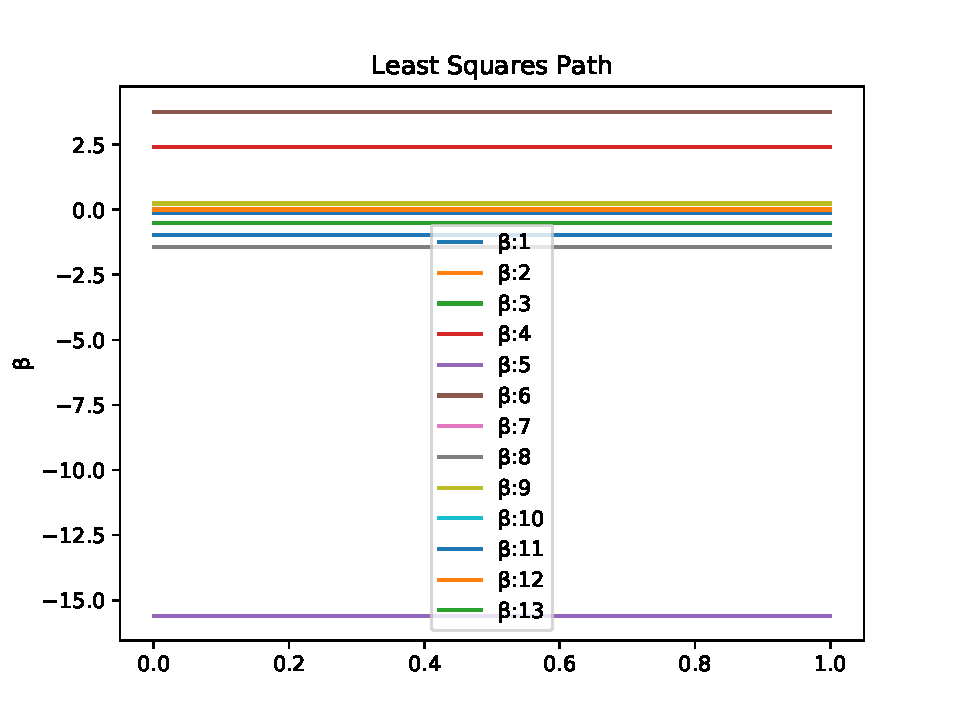
\includegraphics[width=1.0\linewidth]{../img/lrPath.pdf}
                	\caption{最小2乗法の推定値}
               	\label{fig:lr}
    	 \end{minipage}
    	 \begin{minipage}{0.5\hsize}
       		 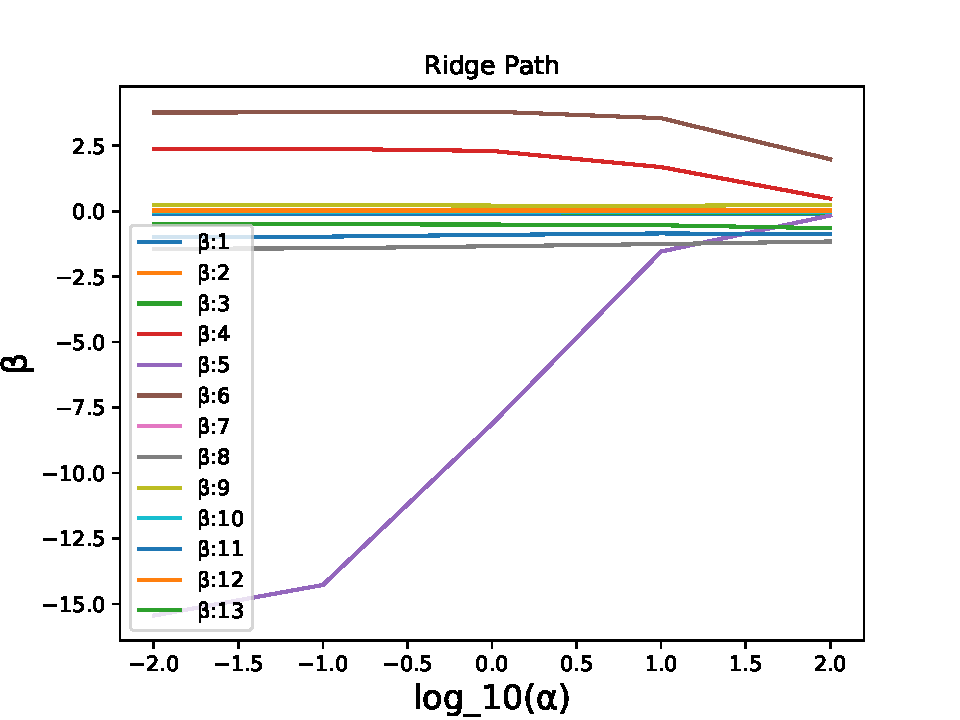
\includegraphics[width=1.0\linewidth]{../img/ridgePath.pdf}
    		 \caption{Ridgeの解パス}
    		 \label{fig:ridge}
    	 \end{minipage}
	     \end{tabular}
\end{figure}

\begin{figure}[H]
    \begin{tabular}{cc}
    	 \begin{minipage}{0.5\hsize}
       		 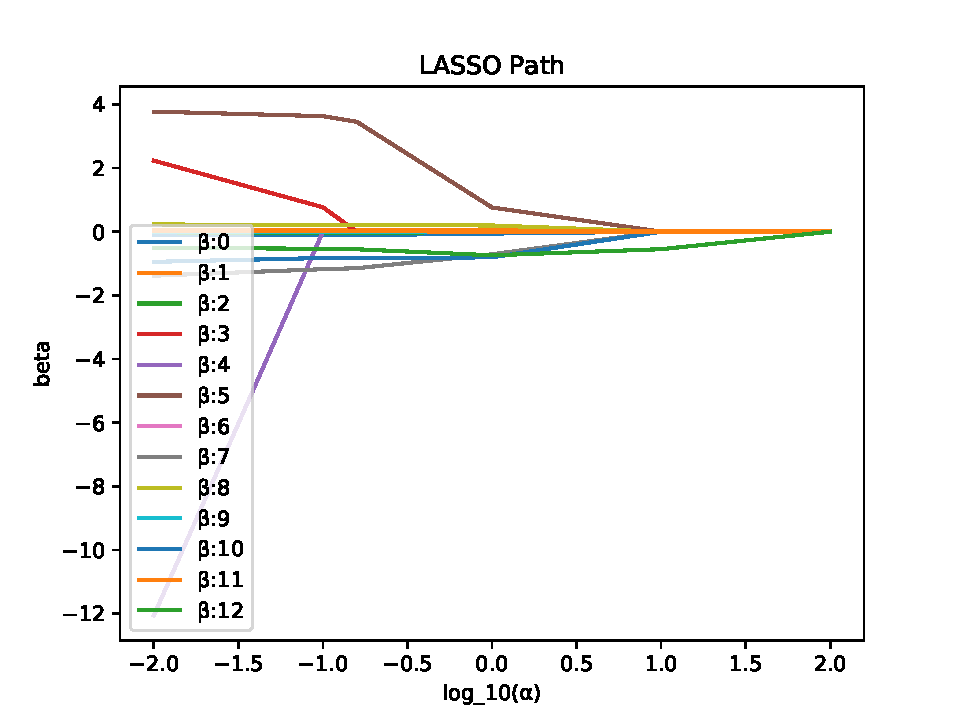
\includegraphics[width=1.0\linewidth]{../img/lassoPath.pdf}
    		 \caption{Lassoの解パス}
    		 \label{fig:lasso}
    	 \end{minipage}
	  \begin{minipage}{0.5\hsize}
                	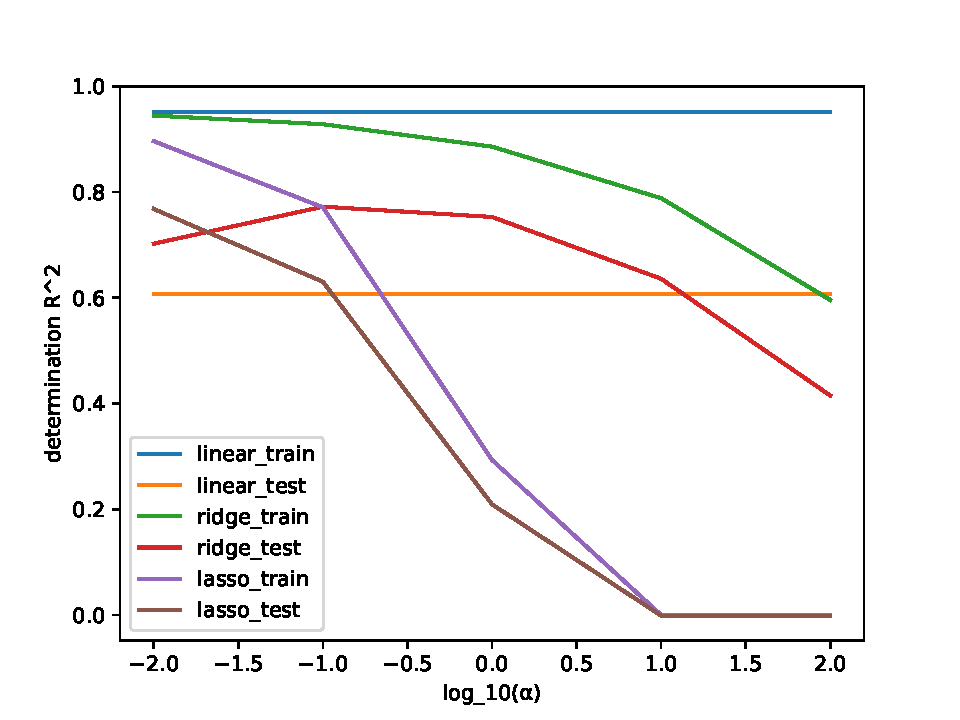
\includegraphics[width=1.0\linewidth]{../img/score.pdf}
                	\caption{決定係数}
               	\label{fig:score}
    	 \end{minipage}
	\end{tabular}
\end{figure}

\begin{table}[H]
	\centering
	\caption{決定係数}
        	\begin{tabular}{|c|c|c|c|c|c|}
		\hline
        		$\alpha$ & 0.01 & 0.1 & 1 & 10 & 100\\ 
		\hline
		\hline
		\multicolumn{6}{|c|}{train} \\
		\hline
		linear & \multicolumn{5}{|c|}{0.95} \\
		\hline
		ridge & 0.94 & 0.93 & 0.89 & 0.79 & 0.60 \\
		\hline
		lasso & 0.90 & 0.77 & 0.29 & 0.00 & 0.00\\
		\hline
		\hline
		\multicolumn{6}{|c|}{test} \\
		\hline
		linear & \multicolumn{5}{|c|}{0.61} \\
		\hline
		ridge & 0.70 & 0.77 & 0.75 &0.64 & 0.42\\
		\hline
		lasso & 0.77 & 0.63 & 0.21 & 0.00 & 0.00 \\
		\hline
        	\end{tabular}
	\label{tab:score}
\end{table}
\section{まとめ}
RidgeとLassoを中心に,正則化法や線形回帰モデルについて学ぶことができた.数式だけでなく,Pythonのパッケージを用いた計算機実験による可視化を通して,自分の中でさらにイメージを具体化させることができた.

今後は,Lassoの計算に用いるアルゴリズムを理解して,パッケージを使わずに実装することが課題である.
\begin{thebibliography}{9}
\bibitem{SK} 小西貞則, 『多変量解析入門』. 岩波書店, 2009.
\end{thebibliography}


\end{document}










